\documentclass[tikz,border=10pt]{standalone}
\usepackage{amsmath}
\usetikzlibrary{arrows.meta, positioning, calc, fit, decorations.pathreplacing}

\definecolor{c1}{HTML}{000000}  % black       - structure, axes
\definecolor{c2}{HTML}{233D4D}  % deep slate  - tokens and rows
\definecolor{c3}{HTML}{FE7F2D}  % orange      - the measurements themselves
\definecolor{c4}{HTML}{EAECF0}  % cool grey   - panel fills
\definecolor{axiscolor}{HTML}{333333}
\definecolor{labelcolor}{HTML}{5F6B75}

\begin{document}
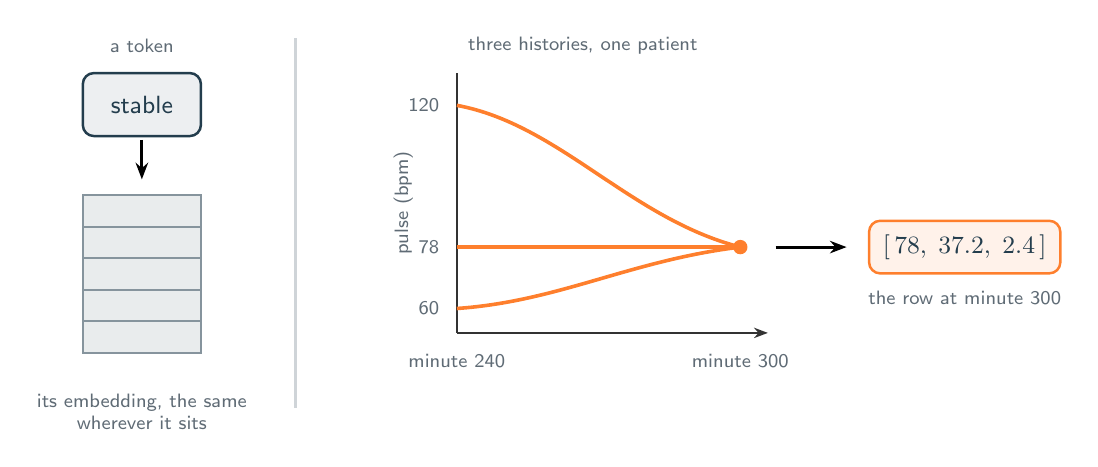
\begin{tikzpicture}[
    every node/.style={font=\sffamily},
    tok/.style={
        rectangle, rounded corners=4pt, minimum width=1.5cm,
        minimum height=0.8cm, line width=0.9pt,
        draw=c2, fill=c2!8, text=c2, font=\sffamily\small,
    },
    cell/.style={
        rectangle, minimum width=1.5cm, minimum height=0.40cm,
        line width=0.7pt, draw=c2!55, fill=c2!10,
    },
    row/.style={
        rectangle, rounded corners=4pt, draw=c3, fill=c3!10, text=c2,
        line width=0.9pt, font=\sffamily\small, inner sep=5pt,
    },
    arr/.style={-{Stealth[length=6pt]}, line width=1.1pt, color=c1},
    lab/.style={font=\sffamily\scriptsize, text=labelcolor},
]

% ================================================ left: one token
\node[lab] at (1.40, 5.35) {a token};
\node[tok] (word) at (1.40, 4.60) {stable};
\draw[arr] (1.40, 4.15) -- (1.40, 3.65);
\foreach \i in {0,...,4}{
    \node[cell] at (1.40, {3.25 - \i*0.40}) {};
}
\node[lab, anchor=north, align=center] at (1.40, 1.05)
    {its embedding, the same\\ wherever it sits};

% divider
\draw[c2!22, line width=0.8pt] (3.35, 0.75) -- (3.35, 5.45);

% ================================================ right: three histories
\node[lab] at (7.00, 5.35) {three histories, one patient};

% axes
\draw[axiscolor, line width=0.8pt] (5.40, 1.70) -- (5.40, 5.00);
\draw[axiscolor, line width=0.8pt, -{Stealth[length=5pt]}] (5.40, 1.70) -- (9.35, 1.70);

\node[lab, anchor=east] at (5.30, 4.59) {120};
\node[lab, anchor=east] at (5.30, 2.79) {78};
\node[lab, anchor=east] at (5.30, 2.01) {60};
\draw[c2!25, line width=0.5pt, dashed] (5.40, 2.79) -- (9.00, 2.79);

\node[lab, anchor=north] at (5.40, 1.55) {minute 240};
\node[lab, anchor=north] at (9.00, 1.55) {minute 300};
\node[lab, rotate=90] at (4.72, 3.35) {pulse (bpm)};

% the three courses, all arriving at 78
\draw[c3, line width=1.3pt]
    (5.40, 4.59) .. controls (6.70, 4.35) and (7.60, 3.15) .. (9.00, 2.79);
\draw[c3, line width=1.3pt]
    (5.40, 2.01) .. controls (6.70, 2.10) and (7.60, 2.62) .. (9.00, 2.79);
\draw[c3, line width=1.3pt] (5.40, 2.79) -- (9.00, 2.79);
\fill[c3] (9.00, 2.79) circle (2.6pt);

% ================================================ the collapse
\draw[arr] (9.45, 2.79) -- (10.35, 2.79);
\node[row] (r) at (11.85, 2.79) {$[\,78,\; 37.2,\; 2.4\,]$};
\node[lab, anchor=north] at (11.85, 2.35) {the row at minute 300};

\end{tikzpicture}
\end{document}
